\documentclass[12pt,a4paper,twoside]{article}
\usepackage{labor}
\begin{document}

%fill for cover and header creation
\newcommand\laboratorynumber{2}
\title{Abbe-Theorie}
\newcommand\supervisor{Robert Nuster}
\newcommand\groupnumber{42}

\newcommand\participantonelastname{Eisner}
\newcommand\participantonefirstname{Nico}
\newcommand\participantoneid{12214121}
\newcommand\participanttwolastname{Waldl}
\newcommand\participanttwofirstname{Philip}
\newcommand\participanttwoid{12214120}
\author{\participantonelastname \ \& \participanttwolastname}

\newcommand\degreeid{UB 033 678}
\newcommand\semester{23WS}
\date{01.12.2023}

%select correct course title
%\newcommand\coursetitle{Einführung in die \\ physikalischen Messmethoden}
%\newcommand\coursetitle{Laborübungen 1: \\ Mechanik und Wärme}
\newcommand\coursetitle{Laborübungen 2: \\ Elektrizität, Magnetismus, Optik}
%\newcommand\coursetitle{Fortgeschrittenen Praktikum 1: \\ Technische Physik}
%\newcommand\coursetitle{Fortgeschrittenen Praktikum 2: \\ Allgemeine Physik}

%\begin{titlepage}
   \begin{center}
       \begin{figure}[H]
            \begin{minipage}[h]{30mm}
                \centerline{
\includegraphics[height=15mm]{cover_nudes/tugraz.png}}
            \end{minipage}
            \hfill
            \begin{minipage}[h]{30mm}
                \centerline{
\includegraphics[height=15mm]{cover_nudes/nawi_graz.png}}
            \end{minipage}
            \hfill
            \begin{minipage}[h]{30mm}
                \centerline{
\includegraphics[height=15mm]{cover_nudes/uni-graz.png}}
            \end{minipage}
        \end{figure}
        
        \large{\emph{Institut für Experimentalphysik der Technischen Universität Graz \\
        \& Institut für Physik der Universität Graz}} \\
        \vspace{5mm}
        
        {\Huge \textbf{\coursetitle}}
        \vspace{5mm}
        
        {\huge \laboratorynumber: \thetitle}
    \end{center}
    
    \vfill
    
    \begin{table}[H]
        \LARGE
        \centering
        \begin{tabular}{r l}
            Betreuer:       & \supervisor \\
            Gruppennummer:  & \groupnumber \\
            \\
            Name:           & \participantonelastname, \participantonefirstname \\
            Matrikelnummer: & \participantoneid \\
            Name:           & \participanttwolastname, \participanttwofirstname \\
            Matrikelnummer: & \participanttwoid \\
            \\
            Kennzahl:       & \degreeid \\
            Datum:          & \semester \ | \thedate
        \end{tabular}
    \end{table}
    \vspace{4cm}
\end{titlepage}
\clearpage
\setcounter{page}{1}

%\maketitle %short title alternative


\includepdf[pages={1}]{../Deckblätter/Deckblatt_Gitter.pdf}

\tableofcontents
\newpage

\section{Aufgabenstellung} %jo beschreibn wos gmocht host ------------------------------

Der Versuch Abbe-Theorie behandelt, wie aus dem Namen bereits hervorgeht, die gleichnamige Idee von Ernst Abbe, die in erster Linie die von allen Objekten hervorgehenden Beugungseffekte und deren Zusammenhang mit dem Auflösungsverhalten beinhaltet.
Mittels Experiment der Abbe-Theorie soll dies- und einige weitere Eigenschaften dieses Verhaltens nun gezeigt werden.
Die genauen Arbeitsaufträge sehen dabei wie folgt aus:

\begin{itemize}
    \item Vertrautmachen mit dem experimentellen Aufbau
    \item Bestimmung des Auflösungsvermögens einer Linse in Abhängigkeit ihrer numerischen Apertur für
    \begin{itemize}
        \item blaues Licht
        \item rotes Licht
    \end{itemize}
    \item Untersuchung des Zusammenhangs zwischen der Bildauflösung von einem Spaltgitter und der Zahl der transmittierten Beugungsordnungen
    \item  Freies Experimentieren
    \begin{itemize}
        \item Beugungsbild horizontaler Balken
        \item Änderung des Beugungsbild mit dem Abstand der Balken
        \item Grund für Beugungserscheinungen in der Richtung normal zu den Hauptordnungen
        \item Dunkelfeldmikroskopie
        \item Verbindung zu Fourieroptik
    \end{itemize}
\end{itemize}



\section{Voraussetzungen \& Grundlagen} %Grundlagen erklären, Formeln mit erklärung

\subsection{Auflösungsvermögen und numerische Apertur}


\subsection{Variation der numerischen Apertur}


\subsection{Abbesche Abbildungstheorie}



    \begin{equation}
        \label{eq:Müll}
        \centerline{$M=\frac{muell}{malle}$}
    \end{equation}

\section{Versuchsanordnung} %mit skizze kurz beschreiben ------------------------------

    \begin{figure}[H]
        \centering
        %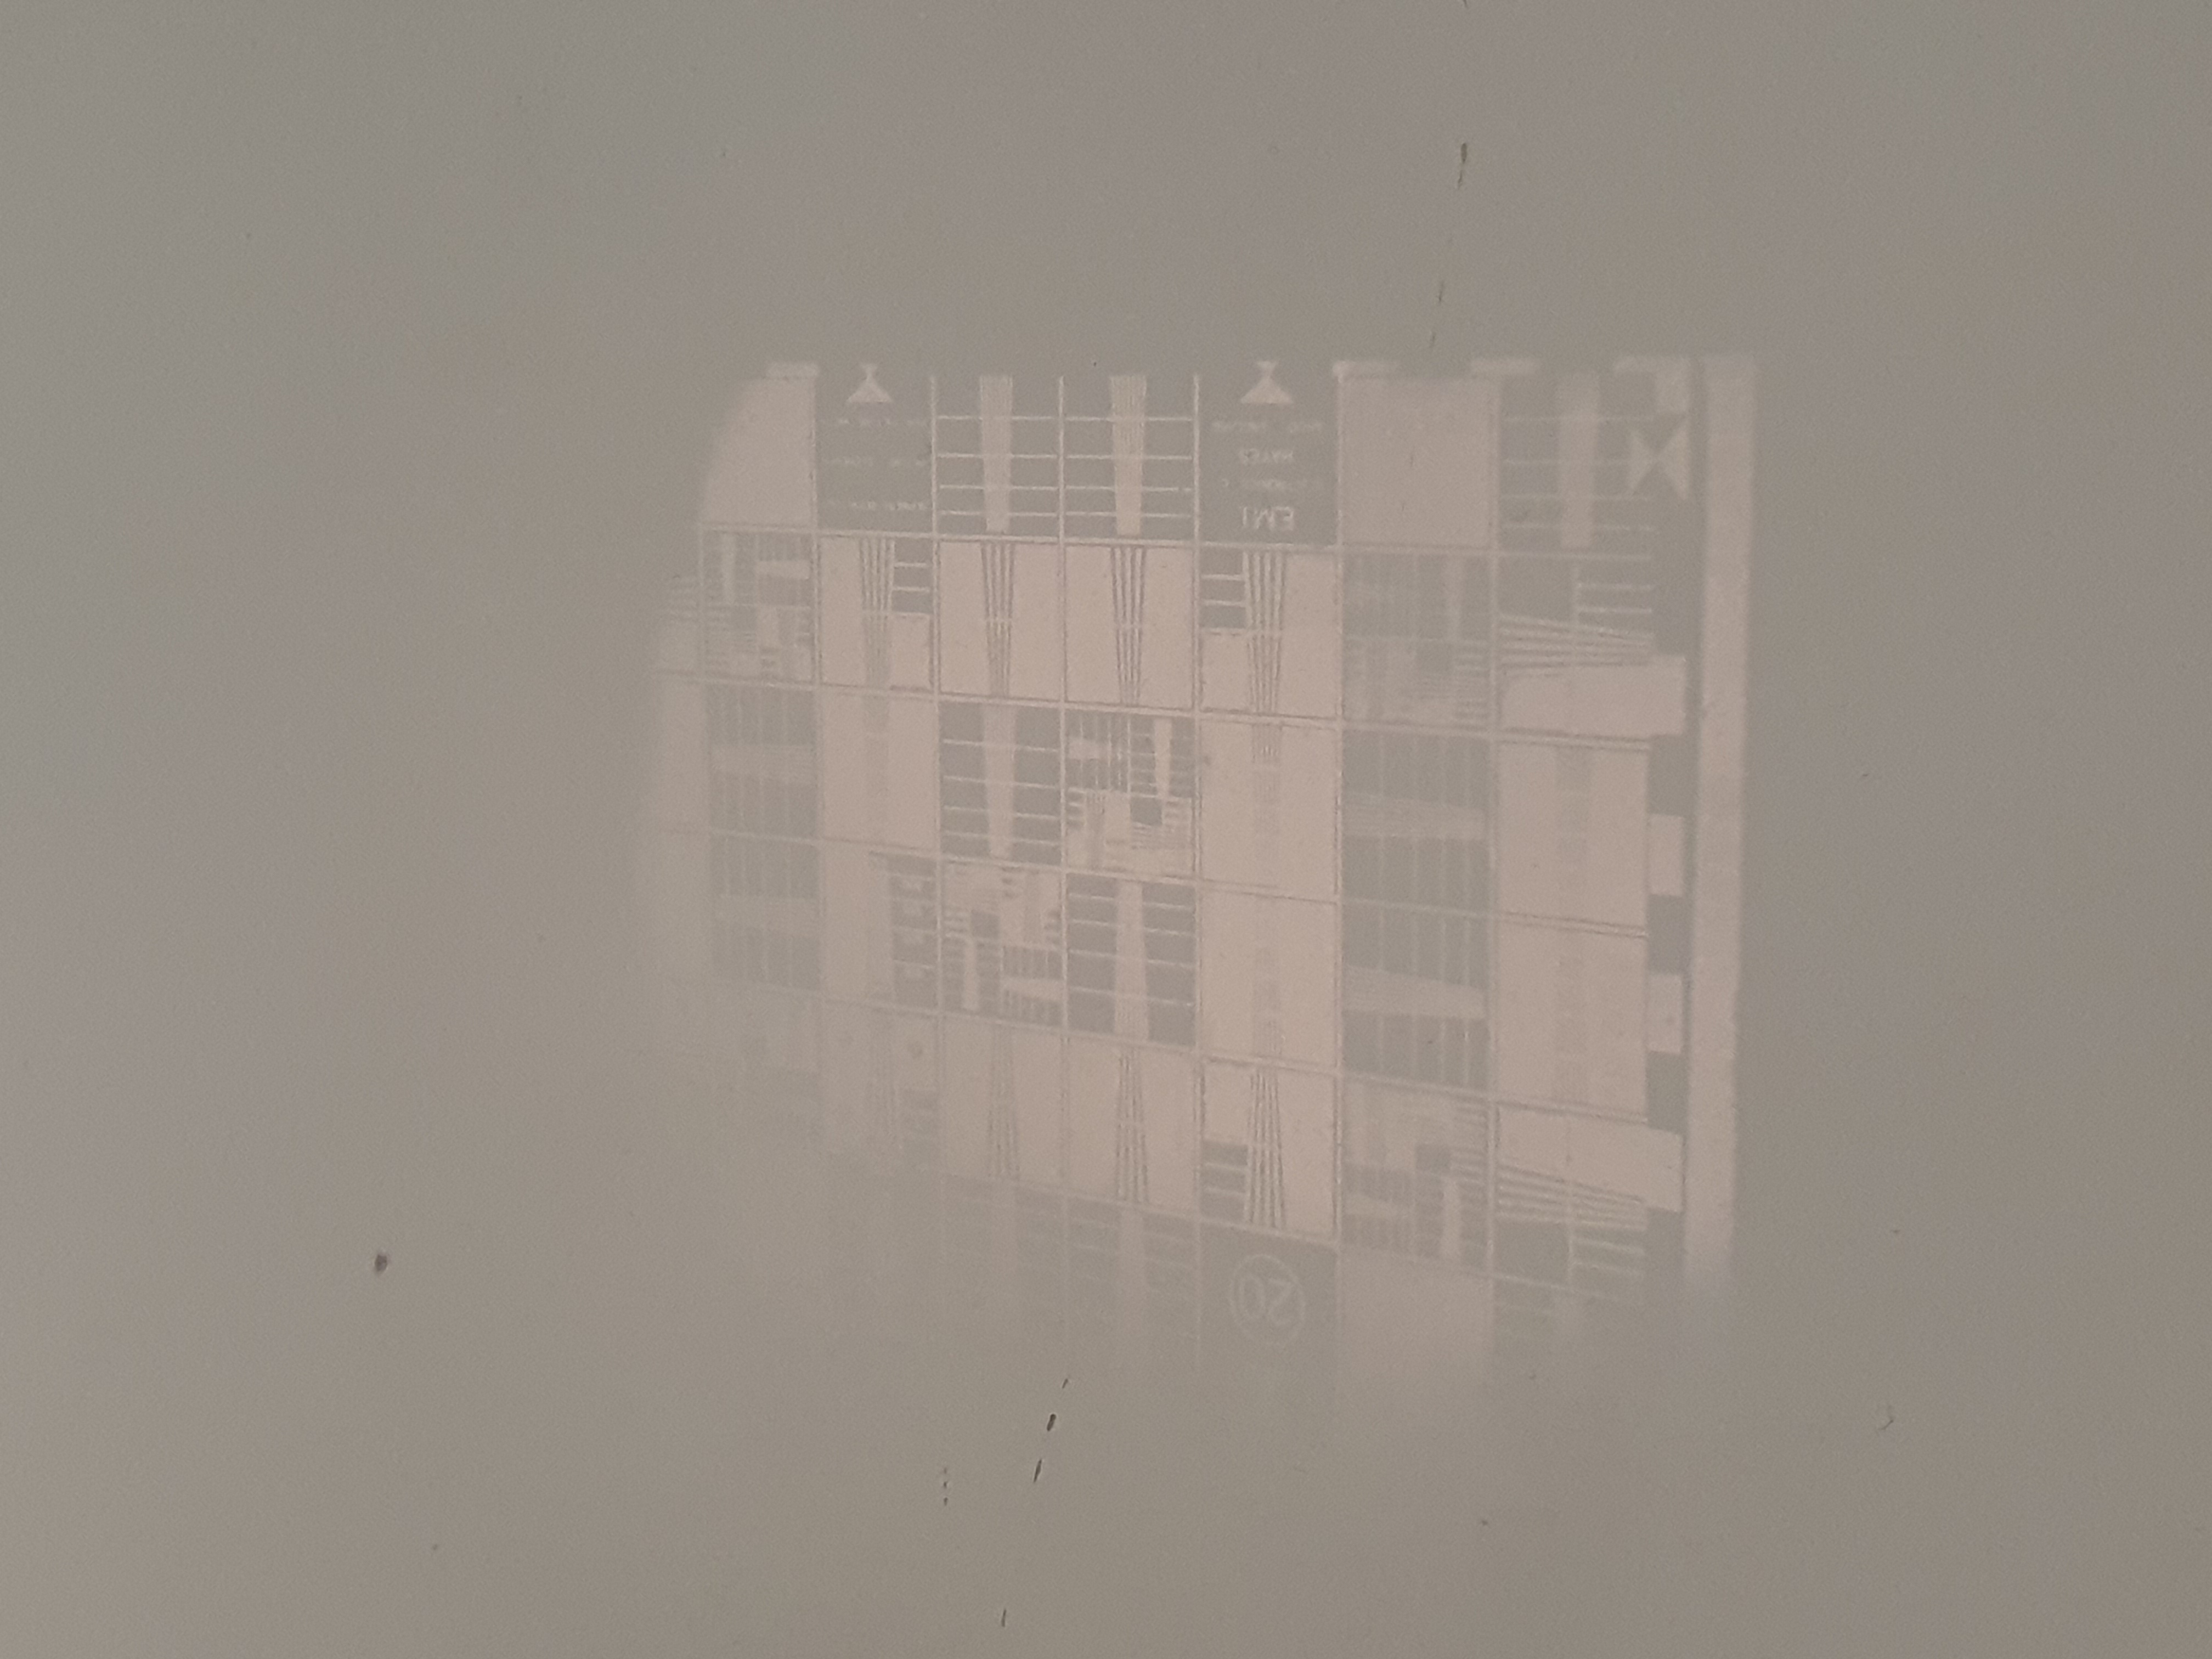
\includegraphics[width=0.6\linewidth, angle=-90]{nudes/bild.jpg}
        \caption{müll}
        \label{fig:müllbild}
    \end{figure}

\section{Geräteliste} %jo holt a listn ------------------------------

    \begin{table}[H]
        \centering
        \caption{Im Versuch verwendete Geräte und Utensilien.}
        \label{tab:geraete}
        \begin{tabular}{| l | l | l | l |}
            \hline
            Gerät   & Typ   & Gerätenummer  & Unsicherheit \\
            \hline
        \end{tabular}
    \end{table}


\section{Versuchsdurchführung \& Messergebnisse} %nachvollziehbar und klar dargestellt ------------------------------


\section{Auswertung und Unsicherheitsanalyse} %Nicht nur zahlen angeben ------------------------------

In der Auswertung werden zur erhöhten Genauigkeit durchgehend ungerundete Werte bis zu den Endergebnissen verwendet und nur zur Darstellung gerundet. \\
Zur Berechnung der Unsicherheiten wird, wenn nicht anders angegeben, die Größtunsicherheitsmethode verwendet.


\section{Diskussion} %diskussion der Unsicherheiten und Ergebnisse und evtl. verlgeich mit Literatur ------------------------------


\section{Zusammenfassung} %klare, übersichtliche vollständige beantwortung der Aufgabenstellung ------------------------------


\printbibliography[heading=bibintoc]
\end{document}
